%\newcommand{\balpha}{\mathbf{\alpha}}

\label{sec:intro}
{
Face hallucination typically refers to the synthesis of a high-resolution (HR) face image from its low-resolution (LR) inputs. Its success would be beneficial for several real-world applications. In this paper, we consider the challenging face hallucination task in which face images might be corrupted due to occlusion. Therefore, our goal is to recover the image pixels of interest in occluded face images.

Given training HR and LR image pairs, most existing face hallucination approaches construct a co-occurrence model for observing the relationships between LR and HR images. Given a test LR image input, the derived model can be directly applied to predict its HR output. Generally, the strategies for performing the above process can be divided into global or local matching based techniques. Global matching based approaches like \cite{eigen, LR} aim to fit the HR image by the LR ones directly. Despite of computation efficiency, such methods might encounter artifacts in the recovered output and thus require additional post processing processes.

\begin{figure}
\graphicspath{{fig/}}
    \begin{center}
        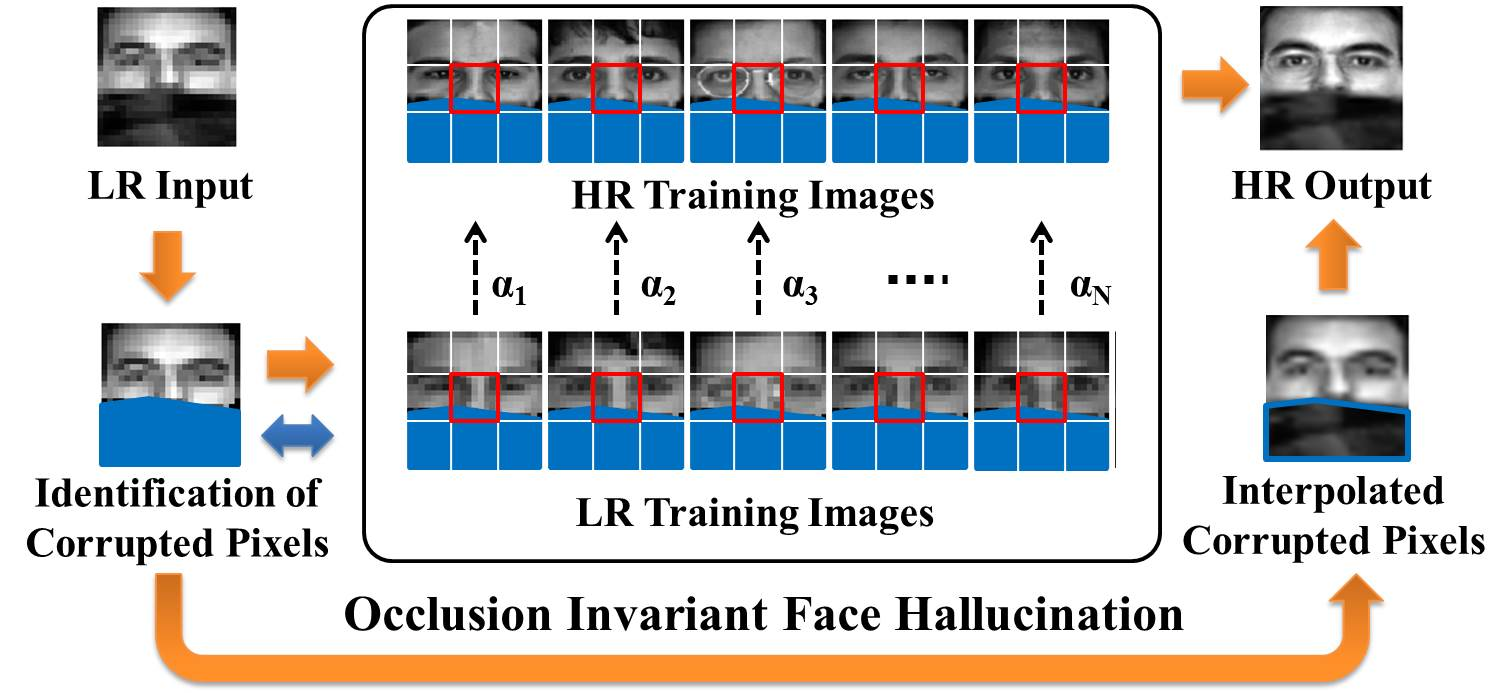
\includegraphics[scale=0.34]{algFlow.jpg}
        \vspace{-0.5cm}
        \caption{\small{Illustration of our proposed framework for occlusion invariant face hallucination. Note that $\alpha$ denotes the coefficient for patch-based image sparse representation.}}
        \label{fig:algFlow}
    \end{center}\vspace{-.5cm}
\end{figure}

On the other hand, local matching based ones perform the above modeling process at the image patch level. Although improved image quality can be achieved, such methods typically involves more sophisticated learning processes. For example, Chang \emph{et al.}~\cite{superRes} proposed a SR framework based on least squares regression (LSR), which selects candidate patches for determining proper reconstruction weights for input image patches. Ma \emph{et al.}~\cite{positionMa} extended the above work by observing the image structure information, and proposed at position-based matching algorithm for face hallucination. Inspired by the above idea, Jung \emph{et al.}~\cite{convex} advocated the sparse representation of such image patches, while Jiang \emph{et al.}~\cite{Jiang_TMM2014} exploited locality information during image synthesis. Recently, coupled-layer information between HR and LR images was further utilized for improved image quality \cite{coupledLayer}.

Nevertheless, the performance of most existing hallucination works would degrade if the input images are corrupted/occluded. To deal with such problems, we propose a sparse representation based scheme for modeling the relationship between HR and LR images in a robust way. To be more specific, our algorithm is able to identify corrupted image pixels during the learning of image representation, which would prevent the degradation of the derived image model by disregarding the poorly reconstructed pixels. As a result, HR images with improved quality will be obtained even if input LR images are corrupted. In our experiments, we will not only show that our method is able to produce satisfactory face hallucination outputs (via both quantitative and qualitative evaluation), we will also confirm that our approach is able to achieve promising recognition results. We will show that our approach would perform favorably against recent approaches on both hallucination and recognition tasks.

%The remaining of this paper is organized as follows. Our proposed LR algorithm for person re-identification will be detailed in Section~\ref{sec:method}. Section~\ref{sec:exp} presents our empirical results, including the comparisons to several baseline and state-of-the-art methods. Finally, Section~\ref{sec:conclusion} concludes this paper.



}
